\section{Aperiodicity via coupling of polyiamond tilings}
\label{sec:coupling}

In this section, we prove the following result:

\begin{theorem}
\label{thm:coupling:aperiodic}
Let $\mathcal{T}$ be a tiling by the hat polykite.  Then $\mathcal{T}$
is not strongly periodic.
\end{theorem}

As noted in \secref{sec:terminology}, a tile that does not admit strongly
periodic tilings also cannot admit weakly periodic tilings.  Therefore,
together with the substitution system outlined in
\secref{sec:discussion}, and described in detail in
Sections~\ref{sec:clusters} and~\ref{sec:subst}, this theorem establishes
that the hat is an
aperiodic monotile, thus proving Theorem~\ref{thm:main}.  The latter
two sections provide a detailed case
analysis showing that all tilings by the
hat polykite are given by the substitution system, and as a
consequence giving an alternative proof that it is an aperiodic
monotile.  Deducing aperiodicity from the result of this section does
not rely on that case analysis, only on the \emph{existence} of
tilings. We require only the description of the substitution system
and the clusters of tiles used in that system, not the proof that all
tilings necessarily obey that system.

We suppose throughout this section that there is a strongly periodic
tiling~$\mathcal{T}$ by the hat polykite, and derive a contradiction.
We also suppose this tiling is aligned to an underlying $[3.4.6.4]$
Laves tiling; this supposition is justified by Lemma~\ref{lemma:tileaalign},
which shows that all tilings by the hat polykite are aligned to such an
underlying Laves tiling.

\begin{figure}
\begin{center}
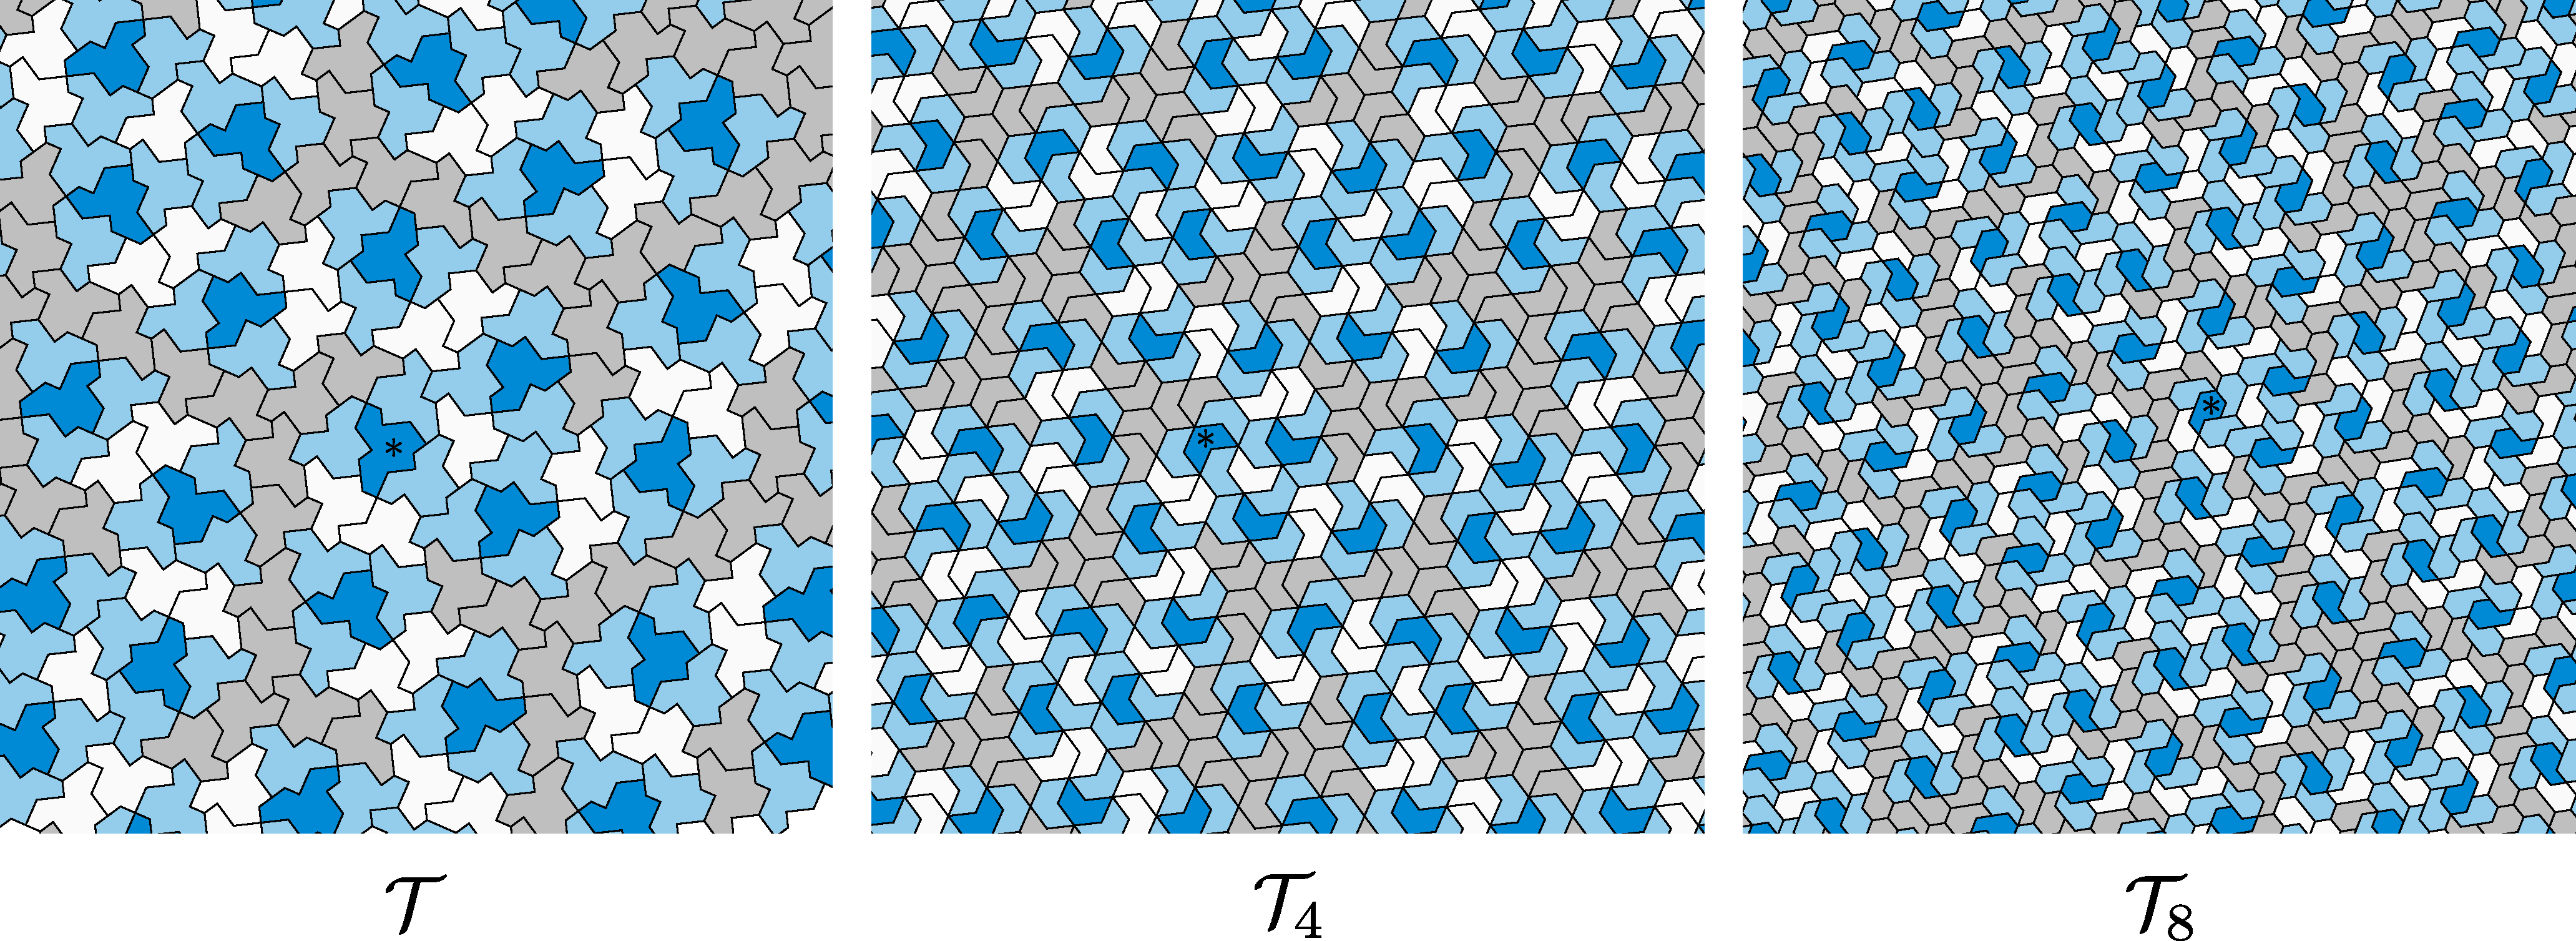
\includegraphics[width=\textwidth]{t_t4_t8.pdf}
\end{center}
\caption{\label{fig:tt4t8}A patch from a hat tiling $\mathcal{T}$ (left),
	which in this section, for eventual contradiction,  is hypothesized to be strongly periodic.  By 
	contracting edges we can construct patches from corresponding 
	$\mathcal{T}_4$ (centre) and $\mathcal{T}_8$ (right) tilings.  Equivalent
	reference tiles are marked with asterisks in the three patches.}
\end{figure}

Contracting the polykite sides of length $1$ or~$2$ to length~$0$
produces a strongly periodic tiling~$\mathcal{T}_4$ by tetriamonds;
contracting the polykite sides of length~$\sqrt{3}$ to length~$0$
produces a strongly periodic tiling~$\mathcal{T}_8$ by octiamonds.
(Because this contraction process is well-defined around any tile,
edge or vertex, it yields a combinatorial tiling of the plane, and a
combinatorial tiling corresponds to a geometrical tiling of the entire
plane~\cite[Lemma~1.1]{regprod}.)  We
suppose that $\mathcal{T}_4$ and $\mathcal{T}_8$ use the same side
lengths as the corresponding sides of the polykite, and have
corresponding tiles in the same orientation.  
\fig{fig:tt4t8} shows a patch from an example tiling $\mathcal{T}$, together
with corresponding patches from $\mathcal{T}_4$ and $\mathcal{T}_8$.
This mapping to tiles of
different side lengths is discussed in more detail in
\secref{sec:family}, where the tetriamond is described as
$\mathrm{Tile}(0,\sqrt{3})$ and the octiamond is described as
$\mathrm{Tile}(1,0)$.

The tilings $\mathcal{T}$, $\mathcal{T}_4$, and $\mathcal{T}_8$ 
are coupled, in the sense that there is a bijection
between their tiles, with corresponding tiles in corresponding
orientations and translation symmetries of any one mapping directly to
translation symmetries of the others.  They also have close combinatorial
relationships: any neighbours in the original
polykite tiling are also neighbours in both polyiamond tilings.  Furthermore,
there must exist affine maps between the lattices of translations of the
$\mathcal{T}_4$ and $\mathcal{T}_8$ tilings, such that
each translation maps to
a corresponding translation (one between corresponding pairs of
tiles).  The affine map sending the translations for~$\mathcal{T}_4$
to those for~$\mathcal{T}_8$ must scale areas by $2/3$.

That affine map cannot be a similarity.  Any distance~$d$ between
vertices of a regular triangular tiling with edge length~$1$ must have
$d^2$ of the form $x^2+xy+y^2$ for integers $x$ and~$y$, and if $2^k
\parallel x^2+xy+y^2$ then $k$~must be even.  Therefore, a scale factor
of~$\sqrt{2}$ is not possible between translations on two triangular
tilings with the same edge length, and a scale factor of~$\sqrt{2/3}$
is not possible between translations on two triangular tilings with
edge lengths $\sqrt{3}$ and~$1$.

Using the fact that the six translation classes of kites must appear
with equal frequency in any aligned tiling by polykites, we now
proceed to show that the affine map from $\mathcal{T}_4$ to 
$\mathcal{T}_8$ must in fact be a similarity, which
gives the required contradiction.

In Figure~\ref{fig:kitetwocol}, we show the hat polykite, with sides
of length $1$ or~$2$ shown as thin \textcolor{\colone}{\textbf{black}}
line segments and sides of length~$\sqrt{3}$ shown as thick
\textcolor{\colroot}{\textbf{orange}} line segments; the two
orientations of kite of which it has two kites (it has exactly one
kite of each other orientation); and the two polyiamonds, in
orientations corresponding to those of the polykite.


\begin{figure}[htp!]
\begin{center}
\begin{tikzpicture}[x=5mm,y=5mm]
  \draw[\colgrid] \vcoords{-1}{-1} -- \vcoords{0}{0} -- \vcoords{4}{-2};
  \draw[\colgrid] \vcoords{0}{0} -- \vcoords{1}{-2} -- \vcoords{2}{-2} --
    \vcoords{2}{0};
  \draw[\colgrid] \vcoords{2}{-2} -- \vcoords{3}{-3} -- \vcoords{2}{-4};
  \draw[\colone] \vcoords{-2}{1} -- \vcoords{-2}{0} -- \vcoords{0}{-2} --
    \vcoords{1}{-2};
  \draw[\colone] \vcoords{4}{-5} -- \vcoords{4}{-4} -- \vcoords{3}{-3};
  \draw[\colone] \vcoords{3}{0} -- \vcoords{2}{0} -- \vcoords{1}{1};
  \draw[\colroot,ultra thick] \vcoords{1}{1}-- \vcoords{0}{0} --
    \vcoords{-2}{1};
  \draw[\colroot,ultra thick] \vcoords{1}{-2} -- \vcoords{2}{-4} --
    \vcoords{4}{-5};
  \draw[\colroot,ultra thick] \vcoords{3}{-3} -- \vcoords{4}{-2} --
    \vcoords{3}{0};
  \draw[\colgrid] \vcoords{6}{-3} -- \vcoords{10}{-5} -- \vcoords{10}{-4} --
    \vcoords{9}{-3} -- \vcoords{7}{-5} -- \vcoords{6}{-4} -- cycle;
  \draw[\colroot,ultra thick] \vcoords{12}{-6} -- \vcoords{14}{-7} --
    \vcoords{15}{-6} -- \vcoords{16}{-8} -- \vcoords{15}{-9} --
    \vcoords{13}{-8} -- cycle;
  \draw[\colone] \vcoords{18}{-9} -- \vcoords{20}{-11} --
    \vcoords{21}{-11} -- \vcoords{21}{-10} -- \vcoords{20}{-9} --
    \vcoords{19}{-9} -- \vcoords{18}{-8} -- cycle;
\end{tikzpicture}
\end{center}
\caption{The hat polykite, its imbalance in kites, and corresponding polyiamonds}
\label{fig:kitetwocol}
\end{figure}

The imbalance in kites of different orientations partitions the twelve
orientations of the hat polykite (that can occur while aligned to an
underlying $[3.4.6.4]$ Laves tiling) into three sets of four, such
that any tiling must have equal proportions of polykites from each set
of orientations (meaning that in any patch with perimeter~$x$, the
imbalance between the numbers of polykites with orientations from any
two of the sets is~$O(x)$).  The same applies to tilings by either
polyiamond derived from tilings by the polykite.  (The tetriamond is
symmetric, so two orientations of the polykite in one of those sets
can give rise to identical-looking tetriamonds.  Those should still be
considered as different orientations of the tetriamond, as if it were
given an asymmetric marking.)

Note that given any two sides of polyiamonds in~$\mathcal{T}_4$, the
corresponding vector in~$\mathcal{T}_8$ between those two sides is
well-defined: a side of a tile in~$\mathcal{T}_4$ corresponds to a
point on the boundary of the corresponding tile in~$\mathcal{T}_8$
(and adjoining sides on adjacent tiles correspond to the same point on
the boundaries of two neighbouring tiles in~$\mathcal{T}_8$), so the
vector is just the vector between those corresponding points.  It is
also convenient for some purposes to divide the tetriamond into two
congruent rhombi, resulting in a tiling~$\mathcal{T}_4'$.  The four
orientations of the tetriamond in one of the three sets of
orientations all contain rhombi in the same two orientations (out of a
possible three), so $\mathcal{T}_4'$~contains equal proportions of
rhombi in each orientation.


\begin{figure}[t]
\begin{center}
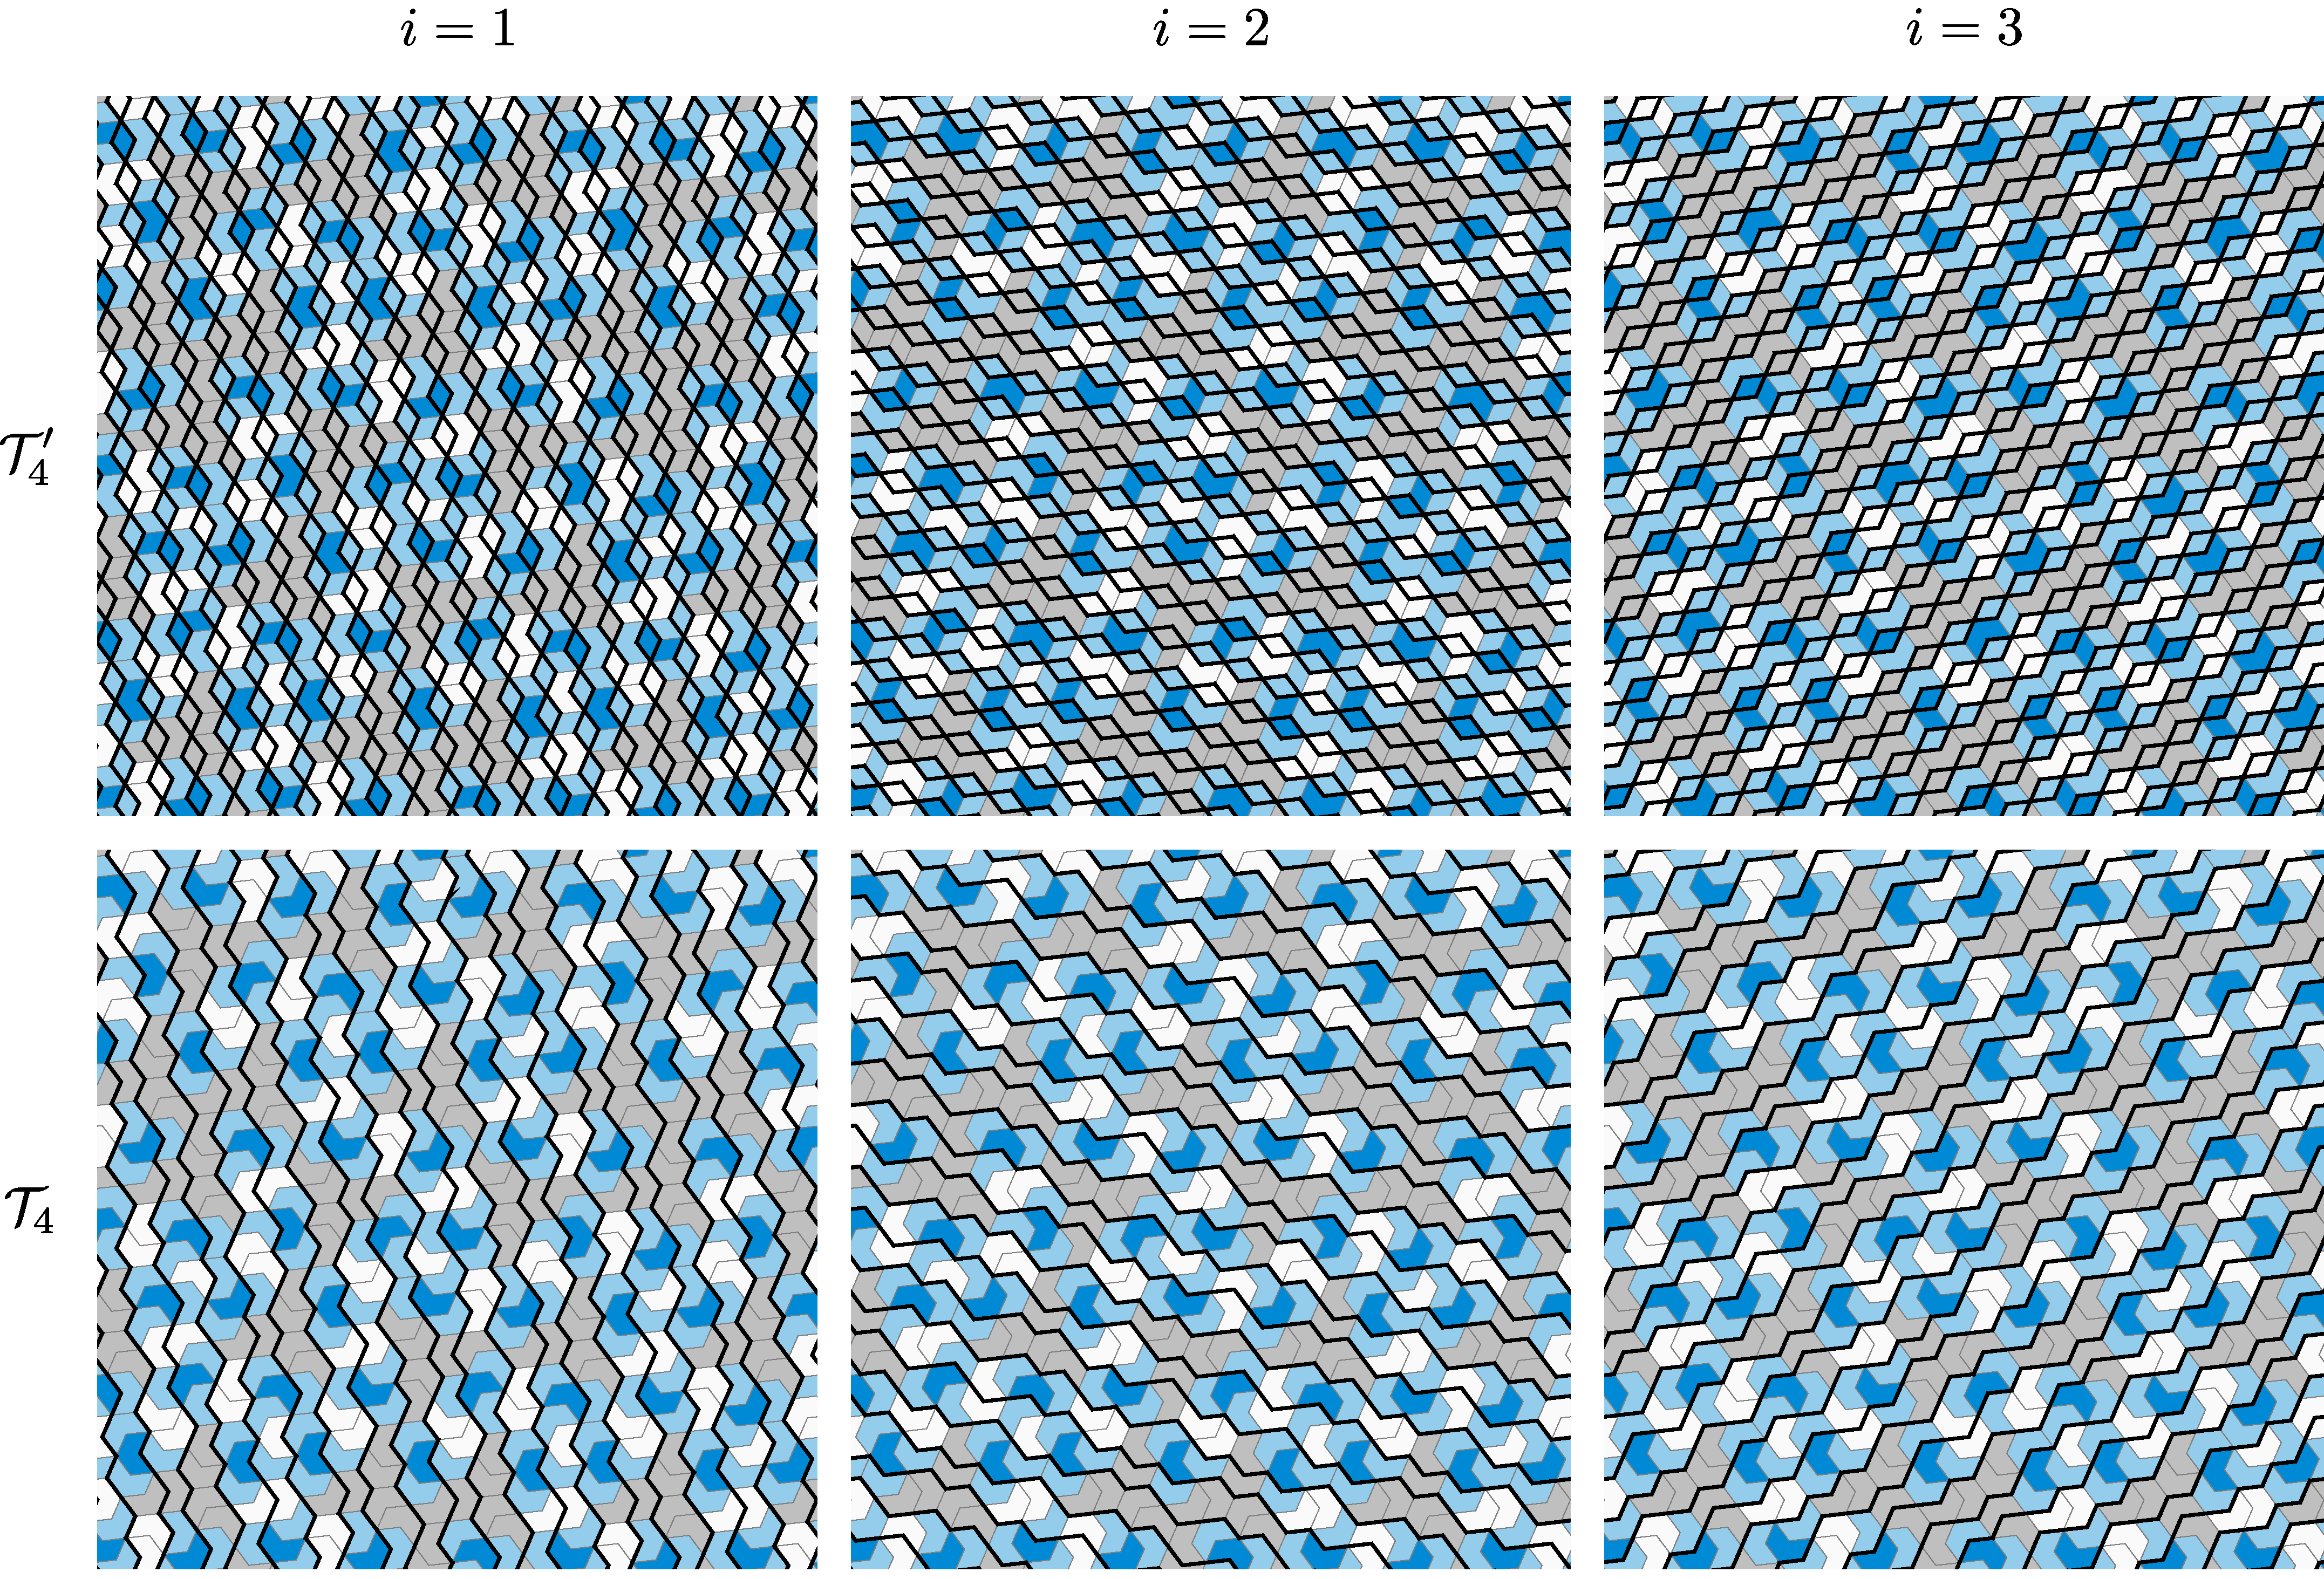
\includegraphics[width=\textwidth]{istrips.pdf}
\end{center}
\caption{\label{fig:istrips}A visualization of the three families of
	$i$-strips in each of $\mathcal{T}_4'$ and $\mathcal{T}_4$, for the 
	sample patch shown in \fig{fig:tt4t8} (centre).  The $i$-strips
	run along the channels between the heavy black boundaries.}
\end{figure}

The edges of the equilateral triangles (of side length~$\sqrt{3}$) in
the regular triangular tiling underlying $\mathcal{T}_4$
and~$\mathcal{T}_4'$ lie in three sets of parallel lines; call those
sets $\mathcal{L}_1$, $\mathcal{L}_2$, and~$\mathcal{L}_3$.  For each
$i\in\{1,2,3\}$, we now form an infinite graph~$\mathcal{G}_i$. 
The vertices of~$\mathcal{G}_i$ are 
those rhombi of~$\mathcal{T}_4'$ that include an edge
lying in some line in~$\mathcal{L}_i$, thereby encompassing rhombi
in two of the three orientations.
Two vertices in $\mathcal{G}_i$ are connected by an edge exactly
when the rhombi corresponding to those vertices are adjacent along an 
edge of~$\mathcal{T}_4'$ lying on some line in~$\mathcal{L}_i$.
The connected
components of this graph are two-way infinite paths, which we refer to
as \emph{$i$-strips} in~$\mathcal{T}_4'$.  
We then partition the tiles of $\mathcal{T}_4$ into a related set of 
$i$-strips by assigning each polyiamond to the same strip as one of its
rhombi.  If a
polyiamond has both rhombi in an orientation that appears in
$i$-strips, they must be in the same $i$-strip, because the line
segment between those two rhombi lies in a line in~$\mathcal{L}_i$.
Note that this assignment must constitute a partition of the tiles
in $\mathcal{T}_4$.
Clearly, the $i$-strips cannot cross, and any line
parallel to those in~$\mathcal{L}_i$ passes through the $i$-strips
in~$\mathcal{T}_4'$ in the same order as any other such line passes
through them.  Furthermore, any translation preserves both $i$-strips
themselves and that ordering of $i$-strips.  \fig{fig:istrips} shows
examples of the three families of $i$-strips for sample patches of
$\mathcal{T}_4'$ and $\mathcal{T}_4$.

Let $\mathbf{v}_i$ be a vector between two consecutive lines
in~$\mathcal{L}_i$, orthogonal to those lines, chosen so the pairwise
angles between those vectors are all~$120^\circ$.  Let $\mathbf{v}'_i$
be a vector orthogonal to~$\mathbf{v}_i$ and with length $1/\sqrt{3}$
times that of~$\mathbf{v}_i$, again chosen so the pairwise angles
between those vectors are all~$120^\circ$.  Note that $\sum_i
\mathbf{v}_i = 0$ and $\sum_i \mathbf{v}'_i = 0$.  Considering the
sides of rhombi in an $i$-strip in~$\mathcal{T}_4'$ that lie in
consecutive lines of~$\mathcal{L}_i$, the vector between the midpoints
of such sides is $\mathbf{v}_i \pm \mathbf{v}'_i$, where the sign
depends on the orientation of the rhombus.  Thus, if the vector
between any two such midpoints is $a \mathbf{v}_i + b \mathbf{v}'_i$,
then between those two sides there are $(a+b)/2$ rhombi of one
orientation and $(a-b)/2$ of the other orientation that can appear in
an $i$-strip in~$\mathcal{T}_4'$.

Considering as symmetries of~$\mathcal{T}_4'$ only those translations
that correspond to translation symmetries of the strongly periodic
tiling~$\mathcal{T}$, there are only finitely many orbits of rhombi
under the action of the group of such translations, so in any
$i$-strip~$\mathcal{S}$ there must be two rhombi in the same orbit.
The translation mapping one to the other is a translation symmetry of
the tiling, and therefore maps $i$-strips to $i$-strips. Because it maps
$\mathcal{S}$ to itself and preserves the ordering of $i$-strips, it
must map every $i$-strip to itself.  If that translation is by a
vector $a \mathbf{v}_i + b \mathbf{v}'_i$, it follows that $b=0$,
because otherwise rhombi of the two orientations that appear in
$i$-strips would appear in the tiling in different proportions.

Thus for each $i$ we have some positive integer~$a_i$, such that a
translation by $a_i \mathbf{v}_i$ is a symmetry of~$\mathcal{T}_4'$
and of $\mathcal{T}_4$ (corresponding to a translation symmetry
of~$\mathcal{T}$, and thus to one of~$\mathcal{T}_8$) that sends each
$i$-strip to itself.  We may replace each~$a_i$ by their lowest common
multiple, so we have a positive integer~$a$ such that for each~$i$ a
translation by $a \mathbf{v}_i$ is a symmetry that sends each
$i$-strip to itself.

We now examine the translation vectors in~$\mathcal{T}_8$
corresponding to $a \mathbf{v}_i$ in~$\mathcal{T}_4$
or~$\mathcal{T}_4'$.  These may be calculated based on the tiles in
any $i$-strip in~$\mathcal{T}_4$ (between any two lines
in~$\mathcal{L}_i$ related by a translation by that vector), and every
$i$-strip (and choice of lines) must produce the same vector
in~$\mathcal{T}_8$.  Figure~\ref{fig:kitetrans} shows the
corresponding translations for three vectors between opposite pairs of
parallel sides of the tetriamond.  For each such pair, first the
vector within the tetriamond is indicated, then the corresponding
octiamond vector as a sequence of octiamond sides, then that vector
decomposed into parts parallel to and orthogonal to the sides between
which the vector is drawn.  Rotating, reflecting or reversing the
direction of the tetriamond vector has the same effect on the
octiamond vector.

\begin{figure}[htp!]
\begin{center}
\begin{tikzpicture}[x=5mm,y=5mm]
  \draw[\colroot,ultra thick] \vcoords{0}{0} -- \vcoords{2}{-1} --
    \vcoords{3}{0} -- \vcoords{4}{-2} -- \vcoords{3}{-3} --
    \vcoords{1}{-2} -- cycle;
  \draw[\colroot,ultra thick,->] \vcoords{3.5}{-1} -- \vcoords{0.5}{-1};
  \draw[\colone] \vcoords{0}{-3} -- \vcoords{2}{-5} --
    \vcoords{3}{-5} -- \vcoords{3}{-4} -- \vcoords{2}{-3} --
    \vcoords{1}{-3} -- \vcoords{0}{-2} -- cycle;
  \draw[\colone,ultra thick,->] \vcoords{2}{-3} -- \vcoords{3}{-4} --
    \vcoords{3}{-5};
  \draw[\colone,ultra thick,->] \vcoords{4}{-4} -- \vcoords{5}{-6};
  \draw[gray] \vcoords{6.5}{-8.25} -- \vcoords{6.5}{-1.25};
  \draw[\colroot,ultra thick] \vcoords{8}{-4} -- \vcoords{10}{-5} --
    \vcoords{11}{-4} -- \vcoords{12}{-6} -- \vcoords{11}{-7} --
    \vcoords{9}{-6} -- cycle;
  \draw[\colroot,ultra thick,->] \vcoords{10.5}{-4.5} -- \vcoords{11.5}{-6.5};
  \draw[\colone] \vcoords{8}{-7} -- \vcoords{10}{-9} --
    \vcoords{11}{-9} -- \vcoords{11}{-8} -- \vcoords{10}{-7} --
    \vcoords{9}{-7} -- \vcoords{8}{-6} -- cycle;
  \draw[\colone,ultra thick,->] \vcoords{8}{-6} -- \vcoords{9}{-7} --
    \vcoords{10}{-7};
  \draw[\colone,ultra thick,->] \vcoords{12}{-8} --
    \vcoords{12.5}{-7.5} -- \vcoords{14}{-9};
  \draw[gray] \vcoords{15}{-12.5} -- \vcoords{15}{-5.5};
  \draw[\colroot,ultra thick] \vcoords{16}{-8} -- \vcoords{18}{-9} --
    \vcoords{19}{-8} -- \vcoords{20}{-10} -- \vcoords{19}{-11} --
    \vcoords{17}{-10} -- cycle;
  \draw[\colroot,ultra thick,->] \vcoords{17}{-8.5} -- \vcoords{18}{-10.5};
  \draw[\colone] \vcoords{16}{-11} -- \vcoords{18}{-13} --
    \vcoords{19}{-13} -- \vcoords{19}{-12} -- \vcoords{18}{-11} --
    \vcoords{17}{-11} -- \vcoords{16}{-10} -- cycle;
  \draw[\colone,ultra thick,->] \vcoords{16}{-10} -- \vcoords{16}{-11}
    -- \vcoords{18}{-13} -- \vcoords{19}{-13};
  \draw[\colone,ultra thick,->] \vcoords{20}{-12} -- \vcoords{23}{-13.5} -- \vcoords{23}{-15};
\end{tikzpicture}
\end{center}
\caption{Corresponding translations for the two polyiamonds}
\label{fig:kitetrans}
\end{figure}

Note that in the first case, the octiamond vector is parallel to the
sides between which the tetriamond vector is drawn; the second and
third cases have equal components orthogonal to those sides.  For the
orthogonal component of the corresponding translations
in~$\mathcal{T}_8$ to be equal for all $i$-strips, it follows that
every $i$-strip must have the same proportion of the second and third
cases relative to the first case.  As the first case corresponds
exactly to one of the three sets of orientations that occur in equal
proportions in any tiling, the first case must thus be a third of the
tetriamonds in any $i$-strip, while the second and third cases (which
together correspond to the other two sets of orientations; however,
each case does not correspond to a single set of orientations) in that
figure must add to two thirds of the tetriamonds.

Since that proportion is independent of~$i$, the orthogonal components
of the translation vectors in~$\mathcal{T}_8$ corresponding to $a
\mathbf{v}_i$ (which are $\frac{a}{2} \mathbf{v}_i$) add to zero.
Since the $a \mathbf{v}_i$ add to zero, the vectors in~$\mathcal{T}_8$
also add to zero, and so their parallel components must also add to
zero.  But $\sum_i b_i \mathbf{v}'_i = 0$ if and only if all the
$b_i$~are equal; say they all equal~$b$.  That means the three
translation vectors in~$\mathcal{T}_8$ (which are $\frac{a}{2}
\mathbf{v}_i + b \mathbf{v}'_i$) are at $120^\circ$~angles to each
other, and so the affine map between lattices of translations is a
similarity, which is a contradiction as discussed above.
